%%%%%%%%%%%%%%%%%%%%%%%%%%%%%%%%%%%%%%%%%
%  WAQTEL Documentation
%  Technical manual
%
%%%%%%%%%%%%%%%%%%%%%%%%%%%%%%%%%%%%%%%%%

%----------------------------------------------------------------------------------------
%	PACKAGES AND OTHER DOCUMENT CONFIGURATIONS
%----------------------------------------------------------------------------------------
\documentclass[Waqtel]{../../data/TelemacDoc} % Default font size and left-justified equations


\begin{document}

\let\cleardoublepage\clearpage
%----------------------------------------------------------------------------------------
%	TITLE PAGE
%----------------------------------------------------------------------------------------
\title{WAQTEL}
\subtitle{Technical manual}
\version{\telmaversion}
\date{\today}
\maketitle
\clearpage

%----------------------------------------------------------------------------------------
%	AUTHORS PAGE
%----------------------------------------------------------------------------------------

%----------------------------------------------------------------------------------------
%	TABLE OF CONTENTS
%----------------------------------------------------------------------------------------


\pagestyle{empty} % No headers

\tableofcontents% Print the table of contents itself

%\cleardoublepage % Forces the first chapter to start on an odd page so it's on the right

\pagestyle{fancy} % Print headers again

\thispagestyle{empty}

\chapter*{Abstract}
This technical manual is mainly based on the translation of the TRACER principle note
``Outil de simulation 1-D MASCARET V7.1. Module de qualité d'eau TRACER. Note de principe''
written by Kamal El Kadi Abderrezzak and Marilyne Luck in 2012
\cite{elkadi_tracer_2012} (ref: EDF R\&D-LNHE H-P73-2011-01786-FR).
It also includes the heat atmosphere exchange subsection of the \telemac{3d} theory guide.

TRACER is the transport and water quality module of the 1D free surface code MASCARET.
TRACER simulates the evolution of several coupled tracers
without retroaction on the flow with respect to hydraulic conditions,
boundary conditions, external sources and biochemical interactions between tracers.\\

This note contains an explanation of the method retained for solving the advection-dispersion equation,
and its application to water quality modeling.

All the processes existing in TRACER were implemented in \telemac{2D} and \telemac{3D} through
a new module called \waqtel between v7.0 and v7.2.
The following water quality modules are described:
\begin{itemize}
\item O$_2$ (dissolved oxygen, organic and ammonia loads),
\item BIOMASS (phytoplankton biomass and nutrients),
\item EUTRO (dissolved oxygen, phytoplankton biomass, nutrients, organic and ammonia loads),
\item MICROPOL (micropollutants and suspended matter),
\item THERMIC (water temperature),
\item degradation law.
\end{itemize}
A reference to the library documentation of the water quality and aquatic ecology model
AED2 is also given.

\newpage

\chapter{Water quality models}
\label{waq_models}
To simplify the document, the operator $F(C)$ is defined as follows:

\begin{equation}
  F(C) = \frac{\partial C}{\partial t} + \vec{U} \cdot \vec \nabla C
       - \nabla \cdot \left( k \vec \nabla C \right),
\end{equation}

with $C(x,y,z,t)$ is the concentration of tracer,
$k$ the coefficient of diffusion (m$^2$/s),
$\vec{U}$ the velocity vector (m/s).\\


In a water quality model, studied substances are advected and dispersed in the mass of water.
Their dispersion in the aquatic environment is linked to transport due to the flow on the one hand
and to the turbulent dispersion of the flow on the other hand.

The concentration of a substance (pollutant, oxygen, etc.) is also influenced by:
\begin{itemize}
\item punctual contributions, caused by releases (factories, sewage treatment plants, etc.)
  which are called \emph{external sources},
\item the presence of other substances in the mass of water, with which the tracer
  may react through biochemical transformations or the existence of forcings
  linked to its own concentration (e.g. the reaeration phenomenon for oxygen).
  These source terms for one tracer are called \emph{internal sources}
  (because internal to the mass of water) and they characterize the water quality module
  (description of the interactions between the tracers).
\end{itemize}

Solving a water quality problem consists in solving a system of $N$ advection-dispersion
equations (one equation per tracer) in which there are
possible external sources (releases, etc.)
and internal sources that exist through biochemical reactions.

A water quality model is characterized in WAQTEL by the coupled treatment of different tracers
and the description of the \emph{internal} source terms.\\

The internal source term for tracer $i$ can be written through the following form:
\begin{equation}
  S_{intern_i} = \lambda_i^0 + \sum_{j=1}^{N} \lambda_i^j C_j + \frac{\mu_i^0}{h}
               + \frac{\sum_{j=1}^{N}\mu_i^j C_j}{h}
\end{equation}

with $\lambda_i^0$ and $\mu_i^0$ the terms not depending on the tracer concentration $i$.

In the above equality, the 1$^{\rm{st}}$ term represents the volumic internal sources
(chemical reactions, etc.) whereas the 2$^{\rm{nd}}$ term represents the surfacic internal sources
(deposition, re-suspension, evaporation, etc.).

Depending on the water quality module, the matrices [$\lambda$] and [$\mu$]
containing the coefficients $\lambda_i^j$ and $\mu_i^j$ will be written differently.
The internal source terms relating water quality processes are treated
in an explicit way in the advection-diffusion equation,
as they depend on the concentration of other tracers,
unknown at the time step $n+1$.

If there are interactions between tracers or specific evolution laws of tracers,
a water quality model can be used to determine the internal sources of tracers
that can be involved in the transport equation.

Internal sources of tracers are computed in the water quality module \waqtel
at each time step, with respect to physical parameters and
the concentrations of different tracers.
Then they are given to \telemac{2d} or \telemac{3d} which compute
the tracer evolution (by advection and diffusion) taking the
source terms into account.\\

Several water quality modules are available in the \waqtel library:
\begin{itemize}
  \item O$_2$ module: simplified model of dissolved oxygen,
  \item BIOMASS module: phytoplankton biomass model,
  \item EUTRO model: eutrophication model (dissolved oxygen and algal biomass),
  \item MICROPOL: model for the evolution of heavy metals or radioelements,
    taking into account their interaction with fine sediments (suspended matter).
    Anyway, no modification of bottom is done,
  \item THERMIC module: model for the evolution of water temperature under the influence
    of atmospheric fluxes,
  \item AED2 model: the water quality and aquatic ecology model,
  \item degradation law.
\end{itemize}

The different modules and their features are described in the following chapters
in which the internal source terms are also detailed.

Note that the structure chosen for \waqtel enables to easily add new
water quality modules, by implementing terms relating to internal sources.


\chapter{O$_2$ Module}

The O$_2$ module is a simple oxygen evolution module,
intermediate between the Streeter and Phelps
\cite{streeter_ohio_1925} model,
which is restricted to modeling reaeration and the global oxidizable load,
and a more complete module, such as EUTRO, simulating several oxidation processes
and explicitly computes the phytoplankton evolution and its influence on oxygen.
The O$_2$ model advantage is its simplicity
(eight parameters to calibrate, excluding parameterization of weirs).
Some important parameters are assumed constant, such as benthic demand or plant respiration.
The use of the model is consequently limited to phenomena of a few days duration,
such as reservoir emptying. Three tracers are involved:

\begin{itemize}
\item dissolved oxygen O$_2$ (mgO$_2$/l),
\item the organic load L (mgO$_2$/l),
\item the ammonia load NH4 (mgH$_4$/l).
\end{itemize}

These variables are advected and dispersed in the water mass accordingly
to the advection-dispersion equation, with external and internal sources.
Six factors influencing the concentration of dissolved oxygen are considered:

\begin{itemize}
\item four factors consuming oxygen: organic load, ammonia load,
  benthic demand and plant respiration,
\item two processes creating oxygen: photosynthesis and reaeration.
\end{itemize}

The terms dealing with internal sources of each considered tracer are explained
in the following sections.

\section{Dissolved oxygen}

\subsection{Benthic demand}

The benthic demand $BEN$ is provided by the user in gO$_2$/m$^2$/d.
It is adjusted according to the temperature $T$ as:

\begin{equation}
  BEN_T = BEN_{20^\circ \rm{C}} (1.065)^{T-20}.
\end{equation}

The following Table gives some typical values of benthic demand
at $T$ = 20$^\circ$C (i.e. $BEN_{20^\circ \rm{C}}$).\\

\begin{table}[H]
 			\centering
\begin{tabular}{p{3.0in}p{3.0in}}
\hline
%row no:1
\multicolumn{1}{|p{3.0in}}{Bottom type} & 
\multicolumn{1}{|p{3.0in}|}{Typical value of $BEN$ (gO$_2$/m$^2$/d) at 20$^{\circ}$C} \\
\hline
%\hhline{--}
%row no:2
\multicolumn{1}{|p{3.0in}}{Filamentous bacteria (10~g/m$^2$)} & 
\multicolumn{1}{|p{3.0in}|}{7} \\
\hline
%\hhline{--}
%row no:3
\multicolumn{1}{|p{3.0in}}{Mud from waste water, near to release} & 
\multicolumn{1}{|p{3.0in}|}{4} \\
\hline
%\hhline{--}
%row no:4
\multicolumn{1}{|p{3.0in}}{Mud from waste water, far from release } & 
\multicolumn{1}{|p{3.0in}|}{1.5} \\
\hline
%\hhline{--}
%row no:5
\multicolumn{1}{|p{3.0in}}{Estuarine silt} & 
\multicolumn{1}{|p{3.0in}|}{1.5} \\
\hline
%\hhline{--}
%row no:6
\multicolumn{1}{|p{3.0in}}{Sand} & 
\multicolumn{1}{|p{3.0in}|}{0.5} \\
\hline
%\hhline{--}
%row no:7
\multicolumn{1}{|p{3.0in}}{Mineral soil} & 
\multicolumn{1}{|p{3.0in}|}{0.007} \\
\hline
%\hhline{--}

\end{tabular}
\end{table}

\subsection{Plant respiration}

The plant respiration $R$ (in mgO$_2$/d/l) is provided by the user.

\subsection{Photosynthesis}

The photosynthesis $P$ (in mgO$_2$/d/l) depends on algae, water depth and light,
with order of magnitude between 0.3 mgO$_2$/l/d and 9 mgO$_2$/l/d
depending on the flow discharge \cite{streeter_ohio_1925}.
In the O$_2$ model, $P$ is provided by the user.

\subsection{Reaeration}

\subsubsection{Natural reaeration}

Reaeration is an oxygen supply through the free surface.
At macroscopic scale, it can be modeled as linearly proportional to ($C_s$ - [O$_2$]),
where $C_s$ is the oxygen concentration at saturation in the water (in mgO$_2$/l)
(Reminder: $C_s$ = 9 mg/l at 20$^{\circ}$C). Therefore:

\begin{equation}
  Reaeration = k_2 \left( C_s - [\rm{O}_2] \right).
\end{equation}

The coefficient $k_2$ (d$^{-1}$) is a parameter with
orders of magnitude indicated in the Table below
(from \cite{tchobanoglous_wq_1985}).\\

\begin{table}[H]
 			\centering
\begin{tabular}{p{3.0in}p{3.0in}}
\hline
%row no:1
\multicolumn{1}{|p{3.0in}}{Type of watercourse} & 
\multicolumn{1}{|p{3.0in}|}{Interval of $k_2$ (d$^{-1}$) at 20$^{\circ}$C} \\
\hline
%\hhline{--}
%row no:2
\multicolumn{1}{|p{3.0in}}{Small ponds and backwaters} & 
\multicolumn{1}{|p{3.0in}|}{0.10-0.23} \\
\hline
%\hhline{--}
%row no:3
\multicolumn{1}{|p{3.0in}}{Sluggish streams and large lakes} & 
\multicolumn{1}{|p{3.0in}|}{0.23-0.35} \\
\hline
%\hhline{--}
%row no:4
\multicolumn{1}{|p{3.0in}}{Large streams of low flow velocity} & 
\multicolumn{1}{|p{3.0in}|}{0.35-0.46} \\
\hline
%\hhline{--}
%row no:5
\multicolumn{1}{|p{3.0in}}{Large streams of normal flow velocity} & 
\multicolumn{1}{|p{3.0in}|}{0.46-0.69} \\
\hline
%\hhline{--}
%row no:6
\multicolumn{1}{|p{3.0in}}{Swift streams} & 
\multicolumn{1}{|p{3.0in}|}{0.69-1.15} \\
\hline
%\hhline{--}
%row no:7
\multicolumn{1}{|p{3.0in}}{Rapids and waterfalls} & 
\multicolumn{1}{|p{3.0in}|}{> 1.15} \\
\hline
%\hhline{--}

\end{tabular}
\end{table}

There are plenty of formulae calculating $k_2$,
which indicates the low level of our understanding of this process.
We can distinguish conceptual formulae,
valid only within limited conditions,
and semi-empirical and empirical formulae
that are valid where conditions are not too far from those of calibration.
Actually, there is little difference between the formulae when the water depth
is between 0.3~m and 3~m.
The O$_2$ model allows using four formulae cited in \cite{mccutcheon_wq_1989}:

\begin{equation}
  k_2 = 5.23 U h^{-1.67} \quad \rm{(Tennessee~Valley~Authority)},
\end{equation}

\begin{equation}
  k_2 = 5.33 U^{0.67} h^{-1.85} \quad \rm{(Owens~et~al.)},
\end{equation}

\begin{equation}
  k_2 = 0.746 U^{2.695} h^{-3.085} J^{-0.823} \quad \rm{(Churchill~et~al.)},
\end{equation}

\begin{equation}
  k_2 = 3.9 U^{0.5} h^{-1.5} \quad \rm{(O’Connor~and~Dobbins)},
\end{equation}

with $U$ is the magnitude of velocity (in m/s)
and $J$ is the energy slope (in m).

The O’Connor and Dobbins formula provides the best results for shallow rivers.
For deep and rapid rivers, Churchill et al.'s formula is preferable.
Figure \ref{validity_domain_reaeration} shows the areas of application for selected formulae
\cite{mccutcheon_wq_1989}:

\begin{figure}[H]
  \centering
  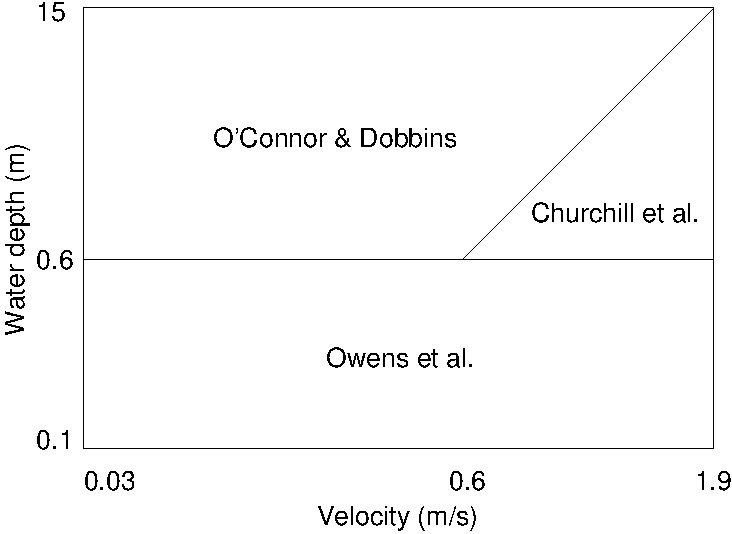
\includegraphics[scale=0.3]{graphics/validity_domain_reaeration_O2.png}
  \caption{Application areas of Owens et al., Churchill et al. and O'Connor
    and Dobbins formulae \cite{mccutcheon_wq_1989}.}
  \label{validity_domain_reaeration}
\end{figure}

One option allows the user fixing a value for $k_2$.
Another option allows choosing one of the four formulae described above.
The value of $k_2$, valid at 20$^{\circ}$C, is adjusted according to the temperature as:

\begin{equation}
  k_2 = (k_2)_{20^{\circ}\rm{C}} (1.0241)^{T-20}.
\end{equation}

The oxygen concentration at saturation in the water $C_s$ can be determined
according to the water temperature (at 20$^{\circ}$C, $C_s$ = 9 mgO$_2$/l).
This is a parameter that must be known and can be calculated
if connected to a temperature module such as THERMIC.
Elmore and Hayes (cited in \cite{mccutcheon_wq_1989}) proposed the following formula
(with $T$ in $^{\circ}$C) for calculating $C_s$:

\begin{equation}
  C_s = 14.652 - 0.41022 T + 0.007991 T^2 - 7.7774.10^{-5}T^3.
\end{equation}

More recent models include a correction for atmospheric pressure and, in estuaries, for salinity.
However, we consider that we are far from estuarial conditions and the variations in pressure
entail insignificant variations in dissolved oxygen compared to those that we need.
Montgomery et al.'s equation (cited in \cite{mccutcheon_wq_1989})
only deviates from standard formulae by $ \pm $  0.02 mgO$_2$/l
between 0 and 50$^{\circ}$C when there is negligible salinity.

\begin{equation}
  C_s = \frac{468}{31.6+T}.
\end{equation}

The model allows choosing either a fixed $C_s$ value given
by the user or by one of the two formulae described above.\\

\subsubsection{Reaeration due to weirs (not used at the moment in WAQTEL)}

A weir can provide between 1 and 3 mg/l of dissolved oxygen \cite{mccutcheon_wq_1989}.
The ratio $r$ is defined by the relationship $$r = \frac{C_s-C_u}{C_s-C_d},$$

with $C_u$ = oxygen concentration upstream of weir,
$C_d$ = oxygen concentration downstream of weir.
The knowledge of $C_u$ and $r$  enables calculating $C_d$.
$C_d$ is directly applied.
This term therefore is not treated as a source.
The rate $r$ can be determined empirically
\cite{mccutcheon_wq_1989}: e.g.,

\begin{equation}
  r = 1 + 0.5 a b \Delta h \quad \rm{(Gameson)},
\end{equation}

\begin{equation}
  r = 1+ 0.36 a b (1+0.046 T) \Delta h \quad \rm{(Gameson~et~al.)},
\end{equation}

\begin{equation}
  r = 1 + 0.69 \Delta h (1 - 0.11 \Delta h) (1 +0.046 T) \quad \rm{(Water~Research~Laboratory)},
\end{equation}

\begin{equation}
  r = 1 + 0.38 a b  \Delta h (1 - 0.11 \Delta h) (1 +0.046 T),
  \quad \rm{(Water~Research~Laboratory)}
\end{equation}

with $a$ = measure of water quality (= 0.65 for highly polluted streams,
= 1.8 for clear streams),
$b$ = characteristic parameter of the weir,
$\Delta h$ = water level difference between upstream and downstream of the weir.
The following Table gives $b$ values for different weirs \cite{mccutcheon_wq_1989}:\\

\begin{table}[H]
 			\centering
\begin{tabular}{p{3.0in}p{3.0in}}
\hline
%row no:1
\multicolumn{1}{|p{3.0in}}{Type of weir} & 
\multicolumn{1}{|p{3.0in}|}{$b$} \\
\hline
%\hhline{--}
%row no:2
\multicolumn{1}{|p{3.0in}}{flat broad-crested regular step} & 
\multicolumn{1}{|p{3.0in}|}{0.7} \\
\hline
%\hhline{--}
%row no:3
\multicolumn{1}{|p{3.0in}}{flat broad-crested irregular step} & 
\multicolumn{1}{|p{3.0in}|}{0.8} \\
\hline
%\hhline{--}
%row no:4
\multicolumn{1}{|p{3.0in}}{flat broad-crested vertical face} & 
\multicolumn{1}{|p{3.0in}|}{0.8} \\
\hline
%\hhline{--}
%row no:5
\multicolumn{1}{|p{3.0in}}{flat broad-crested straight slope face} & 
\multicolumn{1}{|p{3.0in}|}{0.9} \\
\hline
%\hhline{--}
%row no:6
\multicolumn{1}{|p{3.0in}}{flat broad-crested curved face} & 
\multicolumn{1}{|p{3.0in}|}{0.75} \\
\hline
%\hhline{--}
%row no:7
\multicolumn{1}{|p{3.0in}}{round broad-crested curved face} & 
\multicolumn{1}{|p{3.0in}|}{0.6} \\
\hline
%\hhline{--}
%row no:8
\multicolumn{1}{|p{3.0in}}{sharp-crested straight slope face} & 
\multicolumn{1}{|p{3.0in}|}{1.05} \\
\hline
%\hhline{--}
%row no:9
\multicolumn{1}{|p{3.0in}}{sharp-crested vertical face} & 
\multicolumn{1}{|p{3.0in}|}{0.8} \\
\hline
%\hhline{--}
%row no:10
\multicolumn{1}{|p{3.0in}}{sluice gates with submerged discharge} & 
\multicolumn{1}{|p{3.0in}|}{0.05} \\
\hline
%\hhline{--}

\end{tabular}
\end{table}

In the model, $r$ can be either a fixed value given by the user or
calculated by one of the 4 formulae previously described.\\

\section{Organic load}

The organic load $L$ (in mgO$_2$/l) is a variable evolving over time
from an initial condition according to a 1$^{\rm{st}}$ order law:

\begin{equation}
  F([L]) = -k_1 [L],
\end{equation}

where $k_1$ is the kinetic degradation constant of the organic load (d$^{-1}$).
It is a parameter of the model.
In the O$_2$ model, the organic load $L$ is considered to be an independent variable.

\section{Ammonia load}

Also consuming oxygen, the variable ammonia load NH$_4$ (in mgH$_4$/l) follows
a 1$^{\rm{st}}$ order decay law

\begin{equation}
  F([NH_4]) = -k_4 [NH_4],
\end{equation}

where $k_4$ the kinetic constant of nitrification (d$^{-1}$),
a parameter of the model.
In the O$_2$ model, the ammonia load is considered to be an independent variable.\\

\section{Solved equation}

The concentration of dissolved oxygen [O$_2$] (in mgO$_2$/l) changes
according to the effect of sources:

\begin{equation}
  F([O_2]) = k_2 (C_s - [O_2]) -k_1 [L] - k_4 [NH_4] + P - R - \frac{BEN_T}{h}.
\end{equation}

Using the terminology and notations of section \ref{waq_models}
and setting $C_1$ = [O$_2$], $C_2$ = [L] and $C_3$ = [NH$_4$],
the matrices [$ \lambda $] and [$ \mu $]
%containing the coefficients $\lambda_i^j$ and $ \mu_i^j$
are written as:\\

$$  [\lambda] = \frac{1}{86400}
  \begin{pmatrix}
    -k_2 & -k_1  & -k_4 \\
     0   & -k_1  & 0    \\
     0   &  0    & -k_4
  \end{pmatrix}
$$
  
$$
  [\mu] = 
  \begin{pmatrix}
     0  & 0 & 0 \\
     0  & 0 & 0 \\
     0  & 0 & 0
  \end{pmatrix}
$$  

(Note: Division by 86,400 scales down the time to one second).\\

The only non-zeros terms $ \lambda_1^0$ and $ \mu_1^0$ are:

\begin{equation}
  \lambda_1^0 = \frac{k_2 C_s + P - R}{86400},
\end{equation}

\begin{equation}
  \mu_1^0 = -\frac{BEN_T}{86400}.
\end{equation}


\chapter{BIOMASS Module}

The BIOMASS module is a water quality module which allows the calculation of algal biomass.
It estimates the extent of vegetal colonization in terms of various parameters:
sunlight, water temperature, fertilization degree, water renewal ratio,
water turbidity and toxicity \cite{gosse_biomass_1983}.
The BIOMASS module takes into account five tracers:

\begin{itemize}
\item phytoplankton biomass PHY,
\item the principal nutrients influencing its production (phosphorus, nitrogen)
  as well as the associated mineral forms, namely:

\begin{itemize}
\item dissolved mineral phosphorus assimilable by phytoplankton PO$_4$,
\item degradable phosphorus not assimilable by phytoplankton POR,
\item dissolved mineral nitrogen assimilable by phytoplankton NO$_3$,
\item degradable nitrogen not assimilable by phytoplankton NOR.
\end{itemize}
\end{itemize}

These variables are all expressed in mg/l except biomass that is expressed in $\mu$g(Chlorophyl a)/l.\\

We assume these substances acting as tracers,
i.e. they are carried and dispersed in the water mass.
In addition, they react with each other through biochemical processes.\\

The following sections explain the internal source terms.

\section{Phytoplankton}

\subsection{Algal growth}

The algal growth rate $CP$ (d$^{-1}$) is given by:

\begin{equation}
  CP = C_{max} RAY g_1 LNUT \alpha_1,
\end{equation}

with $C_{max}$ = algal growth maximum rate at 20$^{\circ}$C; one can take $C_{max}$ = 2.
$RAY$ represents the effect of sunlight on algal growth;
this dimensionless parameter ranges between 0 and 1;
$g_1$ represents the effect of temperature on algal growth;
$g_1 = T/20$, where $T$ is the water temperature ($^{\circ}$C) (valid for 5$^{\circ}$C < $T$ < 25$^{\circ}$C).
$LNUT$ represents the effects of phosphoric and nitric nutrients on algal growth.
$\alpha_1$ = water toxicity coefficient for algae ($\alpha_1$ = 1 in the absence of toxicity).\\
$RAY$ is calculated by the Smith formula averaged over the vertical:

\begin{equation}
  RAY = \frac{1}{k_e h} \log \left( \frac{I_0 + \sqrt{IK^2+I_0^2} }{ I_h + \sqrt{IK^2+I_h^2} }  \right),
\end{equation}

where $k_e$ is the extinction coefficient of solar rays in water (m$^{-1}$).
It is calculated either by the Secchi depth $Z_s$ using the Atkins formula: $k_e$ = 1.7/$Z_s$, or,
if $Z_s$ is unknown, by the Moss relation: $k_e$ = $k_{pe}$+$ \beta $ [PHY],
where $k_{pe}$ is the coefficient of vegetal turbidity without phytoplankton (m$^{-1}$)
and $ \beta $  the Moss coefficient ($ \beta \approx$ 0.015).
$IK$ is a calibrating parameter (W/m$^2$), of an order of magnitude 100.
$I_0$ is the flux density of solar radiation on the surface (W/m$^2$)
and $I_h$ is the flux density of solar radiation at the bed bottom (W/m$^2$), calculated as:

\begin{equation}
  I_h = I_0 \exp (-k_e h).
\end{equation}

$LNUT$ is calculated by the formula:

\begin{equation}
  LNUT = \min \left( \frac{[PO_4]}{KP+[PO_4]}, \frac{[NO_3]}{KN+[NO_3]} \right),
\end{equation}

with $KP$ = phosphate half-saturation constant (mg/l) (about 0.005 mgP/l),
and $KN$ = nitrate half-saturation constant (mg/l) (about 0.03 mgN/l).\\

Note: Nutrients affect phytoplankton growth PHY only by limiting the factor $LNUT$.
When [PO$_4$] and [NO$_3$] are high enough, $LNUT$ is close to 1 and
phytoplankton evolution no longer depends on nutrients.
In this case, there is no need to model the cycles of phosphorus and nitrogen
for simulating the evolution of phytoplankton.

\subsection{Algal disappearance}

The algal disappearance rate $DP$ (d$^{-1}$) is given as:

\begin{equation}
  DP = (RP+MP) g_2,
\end{equation}

with $RP$ = algal biomass respiration rate at 20$^{\circ}$C (d$^{-1}$),
$MP$ = algal biomass disappearance rate at 20$^{\circ}$C (d$^{-1}$).
$g_2$ represents the effect of temperature on algal disappearance.
$g_2 = T/20$ (valid for 5$^{\circ}$C < $T$ < 25$^{\circ}$C).
$MP$ is given by the following relation:

\begin{equation}
  MP = M_1 + M_2 [PHY] + \alpha_2,
\end{equation}

with $M_1$ and $M_2$ = algal mortality coefficients at 20$^{\circ}$C,
$\alpha_2$ = water toxicity coefficient for algae.

\section{Nitric and phosphoric nutrients}

The following physical and biochemical parameters are used
to describe the processes influencing the evolution of nitric and phosphoric nutrients:

\begin{itemize}
\item $fp$: average proportion of phosphorus in the cells of living phytoplankton (mgP/$\mu$gChlA),
\item $dtp$: proportion of directly assimilable phosphorus in dead phytoplankton ($\%$),
\item $k_1$: transformation rate of POR into PO$_4$ through bacterial mineralization (d$^{-1}$),
\item $k_2$: transformation rate of NOR into NO$_3$ through heterotrophic
  and autotrophic bacterial mineralization (d$^{-1}$),
\item $fn$: average proportion of directly assimilable nitrogen in living phytoplankton (mgN/$\mu$gChlA),
\item $dtn$: proportion of directly assimilable nitrogen in dead phytoplankton ($\%$),
\item $F_{POR}$: deposition flux of non-algal organic phosphorus (g/m$^2$/s).
  $F_{POR} = W_{POR} [POR]$, $W_{POR}$ is the sedimentation velocity of non-algal organic phosphorus (m/s),
\item $F_{NOR}$: deposition flux of non-algal organic nitrogen (g/m$^2$/s).
  $F_{NOR} = W_{NOR} [NOR]$, $W_{NOR}$ is the sedimentation velocity of non-algal organic nitrogen (m/s).
\end{itemize}

Note: sediment transport and resulting bed changes are not modeled in the BIOMASS model.
Deposition is only represented by the deposition flux and,
once organic matter is deposited,
it no longer appears in the equations and can no longer be resuspended.
These deposition fluxes therefore correspond to a definitive loss of mass.

\section{Solved equations}

The BIOMASS model equations are described below, detailing the internal source terms $S_{intern\_i}$.\\

Tracer $\#$1: phytoplankton biomass

\begin{equation}
  F([PHY]) = (CP-DP) [PHY].
\end{equation}

Tracer $\#$2: assimilable mineral phosphorus

\begin{equation}
  F([PO_4]) = fp(dtp DP - CP) [PHY] + k_1 g_2 [POR].
\end{equation}

Tracer $\#$3: non-assimilable phosphorus

\begin{equation}
  F([POR]) = fp(1-dtp) DP [PHY] - k_1 g_2 [POR] - \frac{F_{POR}}{h}.
\end{equation}

Tracer $\#$4: assimilable mineral nitrogen

\begin{equation}
  F([NO_3]) = fn (dtn DP - CP) [PHY] + k_2 g_2 [NOR].
\end{equation}

Tracer $\#$5: non-assimilable nitrogen

\begin{equation}
  F([NOR]) = fn (1- dtn) DP [PHY] - k_2 g_2 [NOR] - \frac{F_{NOR}}{h},
\end{equation}

with $C_1$ = [PHY], $C_2$ = [PO$_4$], $C_3$ = [POR], $C_4$ = [NO$_3$] and $C_5$ = [NOR],
the matrices (5 $\times$ 5) $[\lambda]$ and $[\mu]$
%containing the coefficients $\lambda_i^j$ and $\mu_i^j$
are written as (only non-zero terms are included):

\begin{equation}
\lambda_i^j = \frac{1}{86400}
\left(
%  \begin{array}{c;{2pt/2pt}c;{2pt/2pt}c;{2pt/2pt}c;{2pt/2pt}c}
  \begin{array}{ccccc}
    CP-DP & 0 & 0 & 0 & 0 \\ %\hdashline[2pt/2pt]
    fp (dtp DP -CP) & 0 &  k_1 g_2 & 0 & 0 \\ %\hdashline[2pt/2pt]
    fp (1-dtp) DP   & 0 & -k_1 g_2 & 0 & 0 \\ %\hdashline[2pt/2pt]
    fn (dtn DP -CP) & 0 &        0 & 0 &  k_2 g_2 \\ %\hdashline[2pt/2pt]
    fn (1-dtn) DP   & 0 &        0 & 0 & -k_2 g_2
  \end{array}
\right)
\end{equation}

$$
  \mu_i^j = 
  \begin{pmatrix}
   0 & 0 & 0 & 0 &  0 \\
   0 & 0 & 0 & 0 &  0 \\
   0 & 0 & -W_{POR} & 0 & 0 \\
   0 & 0 & 0 & 0 &  0 \\
   0 & 0 & 0 & 0 & -W_{NOR}
  \end{pmatrix}
$$  

The terms $\lambda_i^0$ and $\mu_i^0$ are zero for every $i$.\\

Divisions by 86,400 are performed to scale down time to one second.


\chapter{EUTRO Module}

The EUTRO module describes the oxygenation of a river.
It is not restricted to modeling reaeration and the global oxidizable load.
It also takes into account the effect of planktonic photosynthesis,
and furthermore models the nitric and phosphoric nutrients and their effect
on phytoplankton (\cite{gosse_doubs_1989} and \cite{gosse_doubs_1983}).\\

This module looks like a combination of the O$_2$ and BIOMASS modules,
except for a more precise treatment of some parameters,
taking into account of the ammonia load in exchanges between nitrogen and phytoplankton,
and of phytoplankton in the calculation of photosynthesis.
More sophisticated than the O$_2$ module, EUTRO requires setting the values of
28 parameters (excluding parameterizing the weirs).\\

It involves 8 tracers:

\begin{itemize}
\item dissolved oxygen O$_2$,
\item phytoplankton biomass (which consumes oxygen through photosynthesis) PHY,
\item the main elements that influence their production
  (phosphorus, nitrogen, ammonia load, organic load)
  as well as the mineral forms associated with phosphorus and nitrogen:
\begin{itemize}
\item dissolved mineral phosphorus assimilable by phytoplankton PO$_4$,
\item degradable phosphorus non-assimilable by phytoplankton POR,
\item dissolved mineral nitrogen assimilable by phytoplankton NO$_3$,
\item ammonia load assimilable by phytoplankton (and consuming oxygen) NH$_4$,
\item degradable nitrogen non-assimilable by phytoplankton NOR,
\item organic load (consuming oxygen) L.
\end{itemize}
\end{itemize}


These variables are expressed in mg/l, except for biomass which is expressed in $\mu$g (Chlorophyll a)/l.\\

The hypothesis assumes these substances to act as tracers,
i.e. they are carried and dispersed in the mass of water.
In addition, they react with each other through biochemical processes.

\section{Processes represented}

Figure \ref{ecosyst_scheme} succinctly presents phenomena modeled\ by the EUTRO model.\\

The following parts show the parameters used and detail internal sources for each of the 8 tracers studied.\\

As with the BIOMASS model, the bottom and the processes which take place there are not modeled in the EUTRO model
(only a deposition flux is taken into account and the quantities deposited no longer appear in the equations).\\

\begin{figure}[H]
  \centering
%  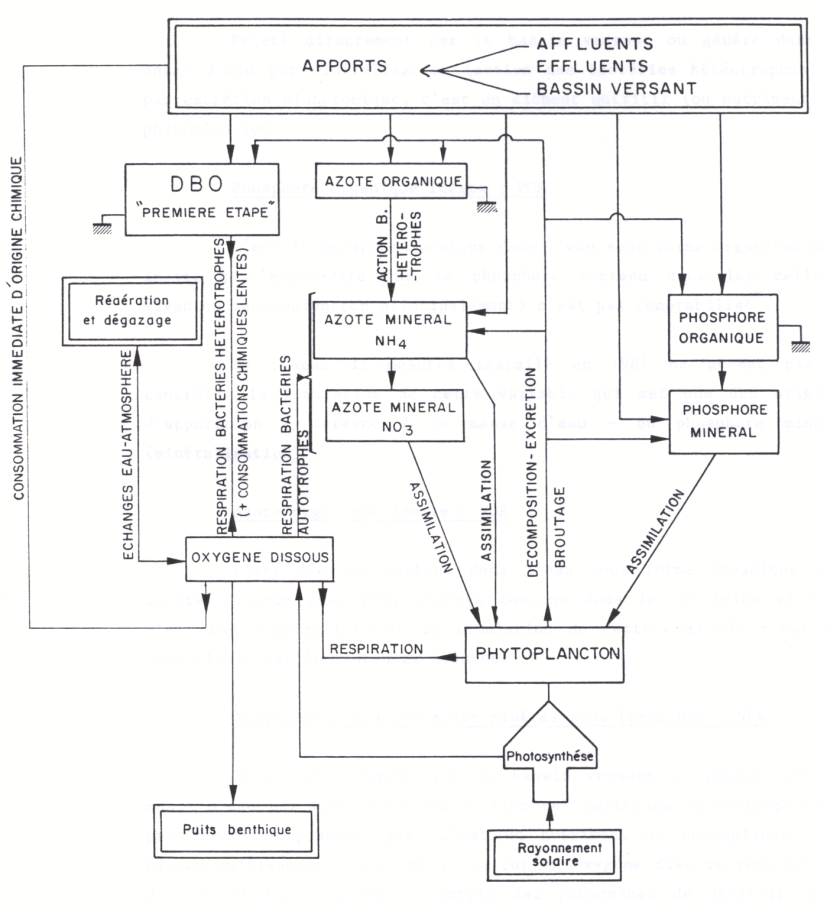
\includegraphics[scale=1.]{graphics/image38.png}
  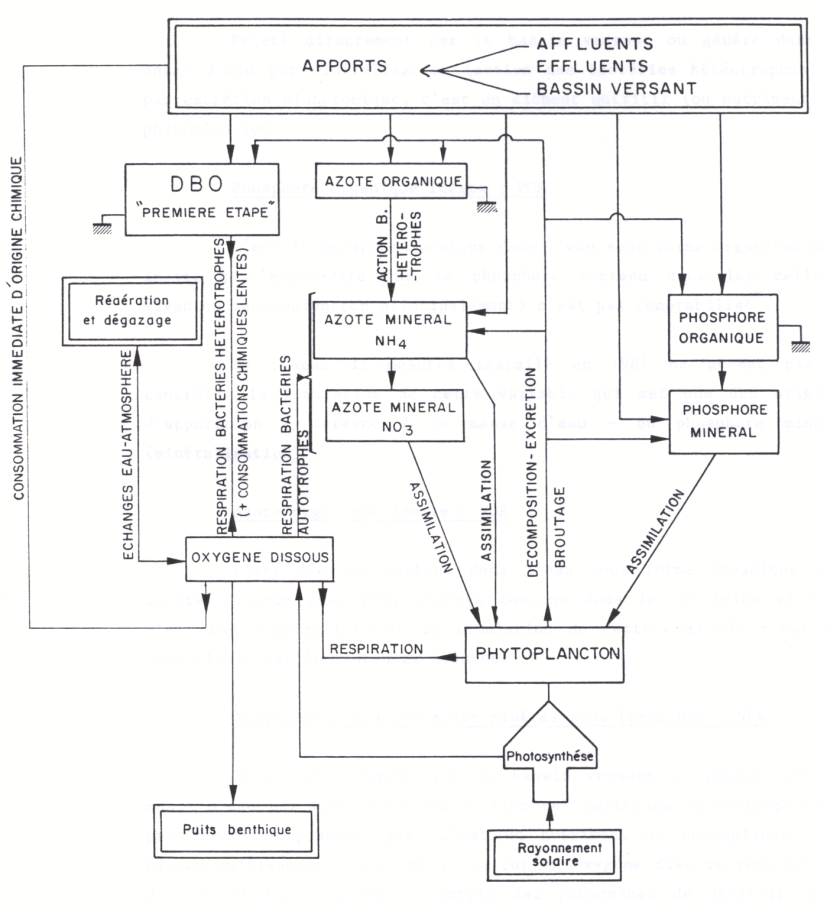
\includegraphics[width=3.76in,height=4.01in]{graphics/image38.png}
  \caption{Schematic representation of the ecosystem modeled by the EUTRO module \cite{gosse_doubs_1989}.
    Figure taken from \cite{elkadi_tracer_2012}.}
  \label{ecosyst_scheme}
\end{figure}

\section{Phytoplankton}

\subsection{Algal growth}

The rate of algal growth $CP$ (d$^{-1}$) is given by the equation:

\begin{equation}
  CP = C_{max} RAY g_1 LNUT \alpha_1.
\end{equation}

The parameters $C_{max}$, $RAY$, $g_1$ and $\alpha_1$ are defined in the same way as in the BIOMASS module.\\

On the other hand, the parameter representing the effects of phosphoric
and nitric nutrients on the algal growth $LNUT$ now takes into account
the ammonia load assimilable by the phytoplankton NH$_4$ and is therefore defined by:

\begin{equation}
  LNUT = \min \left( \frac{[PO_4]}{KP+[PO_4]}, \frac{[NO_3]+[NH_4]}{KN+[NO_3]+[NH_4]} \right),
\end{equation}

with $KP$ the constant of half-saturation in phosphate (mg/l) (about 0.005 mgP/l),
and $KN$ the constant of half-saturation in nitrates (mg/l) (about 0.03 mgN/l).\\

Note: The influence of nutrients on phytoplankton growth PHY is only an intermediate factor limiting $LNUT$.
When [PO$_4$] and [NO$_3$] are big enough, $LNUT$ is close to 1
and phytoplankton evolution no longer depends on nutrients.
In this case, there is no need to model the cycles of phosphorus and
nitrogen in order to simulate the evolution of phytoplankton.

\subsection{Algal disappearance}

The rate of algal disappearance $DP$ (d$^{-1}$) is given by the equation:

\begin{equation}
  DP = (RP + MP) g_2,
\end{equation}

where $RP$ and $MP$ are defined as in the BIOMASS module.
On the other hand, the effect of temperature on algal disappearance
is now represented by the function $g_2$ such that: $g_2 = (1,050)^{T-20}$,
where $T$ is the water temperature ($^{\circ}$C) (valid for 5$^{\circ}$C < $T$ < 25$^{\circ}$C).

\section{Nitric and phosphoric nutrients}

The following physical and biochemical parameters are used to describe processes
influencing the evolution of nitric and phosphoric nutrients:

\begin{itemize}
\item $fp$: average proportion of phosphorus in the cells of living phytoplankton (mgP/$\mu$ChlA),
\item $dtp$: proportion of directly assimilable phosphorus in dead phytoplankton ($\%$),
\item $k_{320}$: rate of transformation of POR into PO$_4$ through bacterial mineralization
  at 20$^{\circ}$C (d$^{-1}$),
\item $k_{620}$: rate of transformation of NOR into NO$_3$ through heterotrophic and autotrophic
  bacterial mineralization at 20$^{\circ}$C (d$^{-1}$),
\item $fn$: average proportion of nitrogen in the cells of living phytoplankton (mgN/$\mu$ChlA),
\item $dtn$: proportion of directly assimilable nitrogen in dead phytoplankton ($\%$),
\item $n$: quantity of oxygen consumed by nitrification (mgO$_2$/mgNH$_4$),
\item $k_{520}$: kinetics of nitrification at 20$^{\circ}$C (d$^{-1}$),
\item $F_{POR}$: deposition flux of non-algal organic phosphorus (g/m$^2$s) = W$_{POR}$.[POR],
  with W$_{POR}$ the sedimentation velocity of non-algal organic phosphorus (m/s),
\item $F_{NOR}$: deposition flux of non-algal organic nitrogen (g/m$^2$s) = W$_{NOR}$.[NOR],
  with W$_{NOR}$ the sedimentation velocity of non-algal organic nitrogen (m/s),
\item $Rn$: proportion of nitrogen assimilated in the form of NH$_4$ = $\frac{[NH_4]}{[NH_4]+[NO_3]}$.
\end{itemize}

\section{Organic load}

The following physical and biochemical parameters are used to describe processes
influencing the evolution of the organic load ($L$):

\begin{itemize}
\item $k_{120}$: constant of the kinetic degradation of the organic load at 20$^{\circ}$C (d$^{-1}$),
\item $g_3$: effect of temperature on degradation of the organic load = $(1.047)^{T-20}$,
  where $T$ is the water temperature ($^{\circ}$C) (valid for 5$^{\circ}$C < $T$ < 25$^{\circ}$C),
\item $F_{LOR}$: deposition flux of the organic load (g/m$^2$s) = $W_{LOR}$.[L],
  with $W_{LOR}$ the sedimentation velocity of the organic load (m/s).
\end{itemize}

\section{Dissolved oxygen}

The following physical and biochemical parameters are used to describe processes
influencing the dissolved oxygen balance (O$_2$):

\begin{itemize}
\item $f$: quantity of oxygen produced by photosynthesis (mgO$_2$/$\mu$gChlA),
\item $BEN$: benthic oxygen demand (gO$_2$/m$^2$/d) (cf. O$_2$ model),
\item $k_2$: coefficient of water-atmosphere gaseous exchange,
  also called coefficient of reaeration, at 20$^{\circ}$C (d$^{-1}$).
  It can be provided by the user or calculated using formulae in the literature (cf. O$_2$ module),
\item $g_4$: effect of temperature on natural reaeration = $(1.025)^{T-20}$,
  where $T$ is the water temperature ($^{\circ}$C) (valid for 5$^{\circ}$C < $T$ < 25$^{\circ}$C),
\item $C_s$: concentration of oxygen saturation in water (mgO$_2$/l).
  It can be determined from the water temperature (cf. O$_2$ module).
%\item $r$: relationship defining the influence of weirs on oxygen concentration (cf. O$_2$ module)
\end{itemize}

\section{Solved equations}

Equations of the EUTRO model are described below:\\

Tracer $\#$1: phytoplankton biomass

\begin{equation}
  F([PHY]) = (CP-DP) [PHY].
\end{equation}

Tracer $\#$2: assimilable mineral phosphorus

\begin{equation}
  F([PO_4]) = fp(dtp DP - CP) [PHY] + k_{320} g_2 [POR].
\end{equation}

Tracer $\#$3: non-assimilable phosphorus

\begin{equation}
  F([POR]) = fp(1-dtp) DP [PHY] - k_{320} g_2 [POR] - \frac{F_{POR}}{h}.
\end{equation}

Tracer $\#$4: assimilable mineral nitrogen

\begin{equation}
  F([NO_3]) = - fn (1- Rn) CP [PHY] + k_{520} g_2 [NH_4].
\end{equation}

Tracer $\#$5: non-assimilable nitrogen

\begin{equation}
  F([NOR]) = fn (1- dtn) DP [PHY] - k_{620} g_2 [NOR] - \frac{F_{NOR}}{h}.
\end{equation}

Tracer $\#$6: ammonia load

\begin{equation}
  F([NH_4]) = fn (dtn DP - Rn CP) [PHY] + k_{620} g_2 [NOR] - k_{520} g_2 [NH_4].
\end{equation}

Tracer $\#$7: organic load

\begin{equation}
  F([L]) = f.MP [PHY] - k_{120} g_3 [L] - \frac{F_{LOR}}{h}.
\end{equation}

Tracer $\#$8: dissolved oxygen

\begin{equation}
  F([O_2]) = f (CP - RP.g_1) [PHY] - n k_{520} g_2 [NH_4] - k_{120} g_3 [L] + k_2 g_4 (C_s - [O_2]) - \frac{BEN}{h}.
\end{equation}

Using the terminology and notations of section \ref{waq_models} and by setting:
$C_1$ = [PHY], $C_2$  = [PO$_4$], $C_3$ = [POR], $C_4$ = [NO$_3$], $C_5$ = [NOR],
$C_6$ = [NH$_4$], $C_7$ = [L], and $C_8$ = [O$_2$],
the matrices (8 $\times$ 8) $[\lambda]$ and $[\mu]$ containing the coefficients
$\lambda_i^j$ and $\mu_i^j$ are written as (only non-zero terms are mentioned):\\

$$  \lambda_i^j = \frac{1}{86400}
  \begin{pmatrix}
    CP-DP               & 0 &            0 & 0 & 0 & 0 & 0 & 0 \\
    fp (dtp DP -CP)     & 0 &  k_{320} g_2  & 0 & 0 & 0 & 0 & 0 \\
    fp (1-dtp) DP       & 0 & -k_{320} g_2  & 0 & 0 & 0 & 0 & 0 \\
   -fn (1 -Rn) CP       & 0 &        0 & 0 & 0 &  k_{520} g_2 & 0 & 0 \\
    fn (1-dtn) DP       & 0 &        0 & 0 & -k_{620} g_2 & 0 & 0 & 0 \\
    fn (dtn DP - Rn CP) & 0 &        0 & 0 &  k_{620} g_2 & -k_{520} g_2 & 0 & 0 \\
    f . MP              & 0 &        0 & 0 & 0 & 0 & -k_{120} g_3 & 0 \\
    f (CP - RP .  g_1 ) & 0 &        0 & 0 & 0 & -n.k_{520} g_2 & -k_{120} g_3 & - k_2 g_4
  \end{pmatrix}
$$  

$$
  \mu_i^j = 
  \begin{pmatrix}
   0 & 0 & 0 & 0 & 0 & 0 & 0 & 0 \\
   0 & 0 & 0 & 0 & 0 & 0 & 0 & 0 \\
   0 & 0 & -W_{POR} & 0 & 0 & 0 & 0 & 0 \\
   0 & 0 & 0 & 0 & 0 & 0 & 0 & 0 \\
   0 & 0 & 0 & 0 & -W_{NOR} & 0 & 0 & 0 \\
   0 & 0 & 0 & 0 & 0 & 0 & 0 & 0 \\
   0 & 0 & 0 & 0 & 0 & 0 & -W_{LOR} & 0 \\
   0 & 0 & 0 & 0 & 0 & 0 & 0 & 0 
  \end{pmatrix}
$$

The only non-zero terms $\lambda_i^0$ and $\mu_i^0$ are:\\

$\lambda_8^0 = \frac{k_2 g_4 C_s}{86400}$ ; $\mu_8^0 = -\frac{BEN}{86400}$

Divisions by 86,400 are performed to scale down time to one second.


\chapter{MICROPOL Module}

The MICROPOL module simulates the evolution of a micropollutant (radioelement or heavy metal)
in the three compartments considered to be of major importance in a river ecosystem:
water, Suspended Particulate Matter (SPM) and bottom material.

It is activated by setting \telkey{WATER QUALITY PROCESS} = 7.\\

Each of these compartments represents an homogeneous class:
SPM and sediments represent the grain-size class of clay and silt
(cohesive fine sediments, of diameter about less than 20 to 25 $\mu$m),
likely to attach the majority of micropollutants.\\

Due to adsorption and desorption of micropollutants,
SPM is one of the first links in the chain of contamination.
SPM is carried and dispersed in the water mass
as a tracer and is also subject to the laws of sedimentary physics:
it settles in calm waters and produces bottom sediments,
and can be re-suspended by a high flow.
Deposits cannot move. They are treated as tracers that can be neither advected
nor dispersed by the water mass, but are likely to be re-suspended.\\

The model considers 5 tracers:

\begin{itemize}
\item suspended matter (SS),
\item bottom sediments (SF), neither advected nor dispersed,
\item dissolved form of micropollutant,
\item the fraction adsorbed by suspended particulate matter,
\item the fraction adsorbed by bottom sediments, neither advected nor dispersed.
\end{itemize}

\subsubsection{Notes, and limitations of the MICROPOL module}

\begin{itemize}
\item whether in suspension or deposited on the bottom, the matter is considered
  to be a passive tracer:
  in other words, it does not influence the flow (no feedback).
  This hypothesis involves that the deposits depth must be negligible compared
  to the water depth (the bed is assumed to be unmodified).
\item there is no direct adsorption/desorption of dissolved micropollutants
  on the deposited matter, only on the SPM
  (the model assumes a preponderance of water – SPM exchanges over direct water
  – bottom sediment exchanges).
  Bottom sediments only become radioactive by means of polluted SPM deposition. 
\end{itemize}

\section{Suspended matter}

The model describing the evolution of SPM and bottom sediments involved in MICROPOL
is a classic representation of the deposition laws and re-suspension
of cohesive SPM, that are the laws of Krone \cite{krone_flume_1962}
and Partheniades \cite{partheniades_erosion_deposition_1965}.\\

Both processes require the knowledge of characteristic constants:

\begin{itemize}
\item deposition occurs when bottom shear stress $\tau_b$,
  which varies according to the flow conditions, becomes lower than a threshold value $\tau_s$,
  known as the critical shear stress for sedimentation
  and which can be set with the keyword \telkey{SEDIMENTATION CRITICAL STRESS}
  (default = 5~Pa) .
  It is then assumed that the SPM settles at a constant velocity $w$
  (known as the settling velocity or velocity of sedimentation)
  with the keyword \telkey{SEDIMENT SETTLING VELOCITY}
  (default = 6.10$^{-6}$~m/s),
\item re-suspension occurs when a threshold $\tau_r$,
  known as the critical shear stress for re-suspension, is exceeded.
  It can be set with the keyword \telkey{CRITICAL STRESS OF RESUSPENSION}
  (default = 1,000~Pa).
  Its importance is weighted by a constant $e$, the rate of erosion characteristic
  of deposited SPM (also known as the Partheniades constant),
  which associated keyword is \telkey{EROSION RATE} (default = 0).
\end{itemize}

\section{Micropollutants}

The model representing the evolution of micropollutants assumes
that the transfers of micropollutants (radioelement, metal)
between the dissolved and particulate phases correspond to either
direct adsorption or ionic exchanges modeled by a reversible reaction,
of 1$^{\rm{st}}$ kinetic order.
%\cite{ciffroy_doubs_1995}.
In the case of direct adsorption, the reaction can be represented in the form of
a reversible reaction, controlled by adsorption ($k_1$ in l/g/s)
and desorption velocities ($k_{-1}$ in s$^{-1}$)
which last associated keyword is \telkey{CONSTANT OF DESORPTION KINETIC}
(default = 2.5 10$^{-7}$~m/s).
It leads to an equilibrium state, and then a distribution of micropollutants
between the dissolved and particulate phase described
by the distribution coefficient $K_d = \frac{k_1}{k_{-1}}$
(set with the keyword
\telkey{COEFFICIENT OF DISTRIBUTION}, default = 1,775~l/g).
Once adsorbed, the fixed micropollutants act like SPM (deposition, re-suspension)
and can also produce areas of polluted sediment.\\

The model includes an exponential decay law (radioactive decay type) of micropollutant
concentrations in each compartment of the modeled ecosystem,
through a constant written $L$
which can be set with the keyword
\telkey{EXPONENTIAL DESINTEGRATION CONSTANT} (default = 1.13 10$^{-7}~\textrm{s}^{-1}$).


\chapter{The THERMIC module}
\label{subs:therm:mod}
For a majority of water quality processes, the interaction with atmosphere is a key parameter.
The THERMIC module is activated by setting \telkey{WATER QUALITY PROCESS} = 11.
The neighboring conditions are taken into account through a meteorological file
like the one described in section \ref{subs:meteo:file}.
It is important to underline that the data contained in this file
can vary depending on the considered case.
The subroutine \telfile{meteo.f} can be edited by the user to customize it to his specific model.

The evolution of temperature of water is tightly linked to heat fluxes through the free surface.
These fluxes (in W/m$^2$) are of 5 natures:

\begin{itemize}
\item sun ray flux $RS$,
\item atmospheric radiation flux $RA$,
\item free surface radiation flux $RE$,
\item heat flux due to advection $CV$,
\item heat flux due to evaporation $CE$.
\end{itemize}

The final balance of (surface) source terms is given by:
\[S_{surf}=RS+RA-RE-CV-CE\]
We will give a brief description for each of these terms, for more details see \cite{El-Kadi2012}.
This surface source term is treated explicitly in \telemac{2d},
the following term is added in the explicit source term of advection-diffusion equation
of tracer$\frac{S_{surf}}{\rho C_pH}$.


\section{Sun ray flux RS}

Sun ray flux is simply provided in the \telkey{ASCII ATMOSPHERIC DATA FILE}.
In a majority of cases, when no measurements are available,
this flux is estimated using the method of Perrin \& Brichambaut (\cite{El-Kadi2012}),
which uses the cloud cover of the sky that varies during the day (function of time).
So far, this flux is considered constant in space.
For more real cases, the user is invited to use the ``heat exchange'' module
(in folder sources/telemac3d).
A sun ray flux varying in space, common between \telemac{2d} and \telemac{3d} will be implemented in next releases.


\section{Atmospheric radiation RA}

The atmospheric radiation $RA$ is estimated with meteorological
data collected at the ground level.
It takes into account energy exchanges with the ground, water
(and energy) exchanges with the underground, etc.
In this module, $RA$ is estimated mainly by the air temperature, like:
\begin{equation*}
RA=e_{air}\sigma\left(T_{air}+273.15 \right)^4\left(1+k\left(\frac{c}{8}\right)^2 \right),
\end{equation*}
where:
\begin{itemize}
\item $e_{air}$ is a calibrating coefficient given by the keyword
  \telkey{COEFFICIENTS FOR CALIBRATING ATMOSPHERIC RADIATION} (default 0.97),
\item $\sigma$ is the constant of Stefan-Boltzmann (= 5.67.10${}^{-8}$ Wm${}^{-2}$K${}^{-4}$),
\item $T_{air}$ is air temperature given in the \telkey{ASCII ATMOSPHERIC DATA FILE},
\item $k$ is the coefficient that represents the nature and elevation of clouds,
it has a mean value of 0.2 (keyword \telkey{COEFFICIENT OF CLOUDING RATE}).
To simplify calculations, an average value of $k$ = 0.2 is usually taken
(default value).
However, it varies like indicated in Table \ref{tab:kcloud}.
\end{itemize}

\begin{table}
  \centering
  \begin{tabular}{|l|c|}
     \hline
     Type of cloud & $k$ \\
     \hline \hline
     Cirrus & 0.04 \\
     Cirro-stratus & 0.08 \\
     Altocumulus & 0.17 \\
     Altostratus & 0.2 \\
     Cumulus & 0.2 \\
     Stratus & 0.24\\
     \hline
   \end{tabular}
  \caption{Values of $k$ depending on cloud type}\label{tab:kcloud}
\end{table}


\section{Free surface radiation RE}

The available water is assumed to behave like a grey body.
Radiation generated by this grey body through the free surface is given by:
\begin{equation*}
RE = e_{water}\sigma\left(T_{water}+273.15 \right)^4,
\end{equation*}
where:
\begin{itemize}
\item $T_{water}$ is the mean water temperature in ${}^\circ$C.
$T_{water}$ is given by the keyword \telkey{WATER TEMPERATURE} (default 7${}^\circ$C),
\item $e_{water}$ is a calibration coefficient which depends on the nature
of the site and obstacles around it.
This coefficient is given with
\telkey{COEFFICIENTS FOR CALIBRATING SURFACE WATER RADIATION} (default 0.97).
For instance, for a narrow river with lots of trees on its banks,
$e_{water}$ is around 0.97, for large rivers or lakes it is about 0.92.
\end{itemize}


\section{Advection heat flux CV}

This flux is estimated empirically:
\begin{equation*}
CV=\rho_{air}C_{p_{air}}\left(a+bV \right)\left(T_{water}-T_{air} \right),
\end{equation*}
where:
\begin{itemize}
  \item $\rho_{air}$ is the air density given by
${\rho }_{air}=\ \frac{100\ P_{atm}}{\left(T_{air}+273.15\right)287}$
where $P_{atm}$ is the atmospheric pressure,
introduced in the \telkey{ASCII ATMOSPHERIC DATA FILE} or using the keyword
\telkey{VALUE OF ATMOSPHERIC PRESSURE} (default 100,000~Pa),
this is a keyword of \telemac{2d} and \telemac{3d},
\item $C_{p_{air}}$ is the air specific heat (J/kg${}^\circ$C)
  given by \telkey{AIR SPECIFIC HEAT} (default 1,005),
\item $V$ is the wind velocity (m/s),
\item $a$, $b$ are empirical coefficients to be calibrated.
Their values are very close to 0.0025, but they can be changed
using \telkey{COEFFICIENTS OF AERATION FORMULA} (default = (0.002, 0.0012)).
\end{itemize}


\section{Evaporation heat flux CE}

 It is given by the following empirical formula:
\begin{equation*}
CE = L(T_{water})\rho_{air}\left(a+bV \right) \left(H^{sat}-H \right)
\end{equation*}
where:
\begin{itemize}
\item $L(T_{water})$ = 2,500,900 - 2,365.$T_{water}$ is the vaporization latent heat (J/Kg),
\item $H^{sat}=\frac{0.622P^{sat}_{vap}}{P_{atm}-0.378P^{sat}_{vap}}$
is the air specific moisture (humidity) at saturation (kg/kg),
\item $H = \frac{0.622P_{vap}}{P_{atm}-0.378P_{vap}}$ is the specific humidity of air (kg/kg),
\item $P_{vap}$ is the partial pressure of water vapour in the air (hPa)
which is given in the \telkey{ASCII ATMOSPHERIC DATA FILE},
\item $P^{sat}_{vap}$ is the partial pressure of water vapour at saturation (hPa) which is estimated with :
\begin{equation*}
P^{sat}_{vap} = 6.11 \exp \left(\frac{17.27T_{water}}{T_{water}+237.3} \right).
\end{equation*}
\end{itemize}

When $H{}^{sat} < H$, the atmospheric radiation $RA$ is corrected by multiplying it with 1.8.



\chapter{AED2 Module}

See the AED2 model technical manual (water quality and aquatic ecology model)
available on the AED2 website:

http://aed.see.uwa.edu.au/research/models/AED/downloads/AED\_ScienceManual\_v4\_draft.pdf


\chapter{Degradation law}

%WAQTEL simulates the evolution of a tracer $C$ over time from an initial condition
%according to a degradation law that is assumed to be of 1$^{\rm{st}}$ order (i.e. a tracer decrease):

%\begin{equation}
%  F([C]) = -k_1 [C],
%\end{equation}

%where $k_1$ is the constant of tracer kinetic degradation $C$ (d$^{-1}$),
%to be specified by the user.

\waqtel can simulate usual laws for bacterial degradation with
$T_{90}$ coefficient(s):
time(s) required for 90\% of the initial bacterial population to disappear
or also described as the time for bacterial or viral concentration to decrease
by one log unit (hence the 2.3 coefficient below).
It is expressed in hours.
%mortality rate(s) of 90~\% when 90~\% of bacteria die.

In other words, it simulates the evolution of tracer(s) $C$ over time from
initial condition(s) according to a degradation law assumed to be of
1$^{\rm{st}}$ order (i.e. a tracer decrease) with constant(s) of tracer kinetic
degradation equal to $\frac{2.3}{T_{90}}$:

\begin{equation}
  F([C]) = -\frac{2.3}{T_{90}} [C],
\end{equation}

with $T_{90}$ coefficient(s) described above, in hours.
%where $T_{90}$ the time when 90~\% of bacteria die, in hours.
\\

\begin{WarningBlock}{Note:}
This is not the evolution of tracer(s) $C$ over time from initial condition(s) 
according to a degradation law that is assumed to be of 1$^{\rm{st}}$ order
(i.e. a tracer decrease):

\begin{equation}
  F([C]) = -k_1 [C],
\end{equation}

where $k_1$ is the constant (or one of the constants) of tracer kinetic
degradation $C$ (d$^{-1}$).
\end{WarningBlock}


\chapter{Conclusion}

WAQTEL simulates the transport of several tracers in a river or the sea
(by resolution of the advection-diffusion equation) possibly coupled
(\textit{via} source terms of the equation).
\waqtel offers a structure that allows programming further water quality modules.\\

This technical manual first shows the method of resolving the convection-dispersion equation
and its application to water quality.\\

The water quality modules available in the WAQTEL tool library are described,
namely:

\begin{itemize}
\item O2: a simplified module for dissolved oxygen,
\item BIOMASS: a module for phytoplankton biomass,
\item EUTRO: a module for river eutrophication (dissolved oxygen and algal biomass),
\item MICROPOL: a module for heavy metals or radioelements,
  taking into account their interaction with fine sediments (suspended particulate matter),
\item THERMIC: a module for water temperature evolution under the influence of atmospheric fluxes,
\item AED2: the water quality and aquatic ecology model,
\item a degradation law.
\end{itemize}

%In the future, the following tasks are expected to be addressed:
%\begin{itemize}
%\item enabling simulation of tracer transport in a hydraulic network that involves floodways,
%\item enabling a distinction to be made between minor riverbeds and major riverbeds
%  in studies of water quality,
%\item finally, taking account of the presence of dead zones (dead/storage zones).
%  This may be useful for river applications during periods of low water. 
%\end{itemize}

%===========================================================================
% Bibliography
%===========================================================================

%\addcontentsline{toc}{section}{References}
\bibliographystyle{plainnat}
%\bibliography{latex/waqtel_theory_guide}

\bibliography{../../data/biblio}

%\printbibliography
\end{document}
